\section{Versuchsaufbau und Versuchsdurchführung}

\begin{flushleft}
    Der Aufbau für diesen Versuch besteht aus einer Kupfer-Röntgenröhre, einem KBr-Kristall, einem Geiger-Müller-Zählrohr und einem Rechner mit dem Programm measure.
    Die Röntgenröhre kann manuell aber auch mit dem Rechner bedient werden, jedoch werden in diesem Versuch alle Messungen mit dem Rechner aufgenommen.
    In dem Programm werden folgende Einstellungen gewählt: \\
    In der oberen Zeile des Programms wird unter dem Menüpunkt Messgerät, Röntgengerät ausgewählt. 
    Unter Messart können Drehmodus, Kristallwinkel, Spektren, Beschleunigungsspannung, Emissionsstrom, Startwinkel sowie Stopwinkel und die Integrationszeit eingestellt werden und die Messung nach einstellen starten.
    Der Emissionsstrom wird dabei durchgehend auf $1\,\unit{\milli\ampere}$ und die Beschleunigungsspannung auf $35\,\unit{\kilo\volt}$ gestellt. 
\end{flushleft}

\begin{figure}[H]
    \centering
    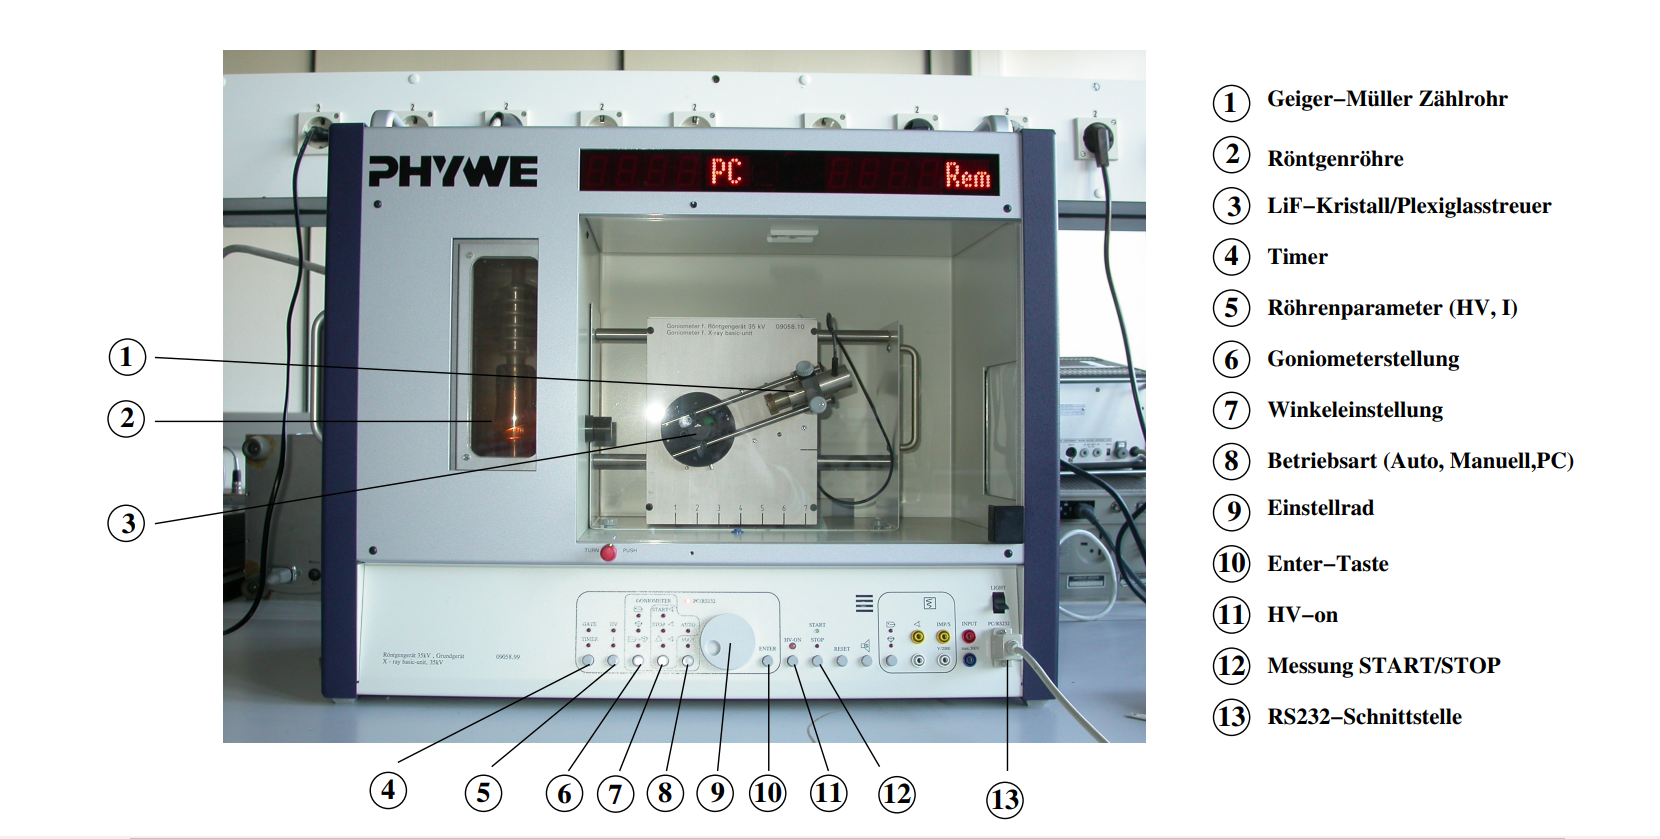
\includegraphics[height=80mm]{bilder/Röntgenröhre.png}
    \caption{Röntgenröhre mit Geiger-Müller-Zählrohr \cite{a1}. \label{Abbildung2} }
\end{figure}

\subsection{Überprüfung der Bragg Bedingung}

\begin{flushleft}
    Um die Bragg Bedingung zu überprüfen wird in dem Programm der Kristall auf einen Festwinkel von $\theta = 14\unit{\degree}$ eingestellt. 
    Der Startwinkel wird auf $\alpha_{\text{Gm}} = 26\unit{\degree}$, der Stopwinkel wird auf $\alpha_{\text{Gm}} = 30\unit{\degree}$, der Winkelzuwachs wird auf $\increment \alpha = 0,1\unit{\degree}$ und die Integrationszeit wird auf $\increment \text{t} = 5\,\unit{\second}$ gestellt.
    Danach kann die Messung gestartet und mit den gemessenen Daten das Maximum der Kurve bestimmt werden.
    Diese wird dann mit dem Sollwinkel verglichen und bei mehr als $1\unit{\degree}$ Unterschied muss der Assistent oder die Praktikumsleitung informiert werden.
\end{flushleft}

\subsection{Das Emissionsspektrum einer Cu-Röntgenröhre}

\begin{flushleft}
    Um das Emissionsspektrum der Kupferröhre zu bestimmen wird unter dem Menüpunkt Messart der 2:1 Koppelmodus ausgewählt, der Startwinkel auf $\alpha = 4\unit{\degree}$ und der Stopwinkel auf $\theta = 26\unit{\degree}$ gesetzt.
    Der Winkelzuwachs wird auf $0,2\unit{\degree}$ und die Integrationszeit auf $\increment t = 5\,\unit{\second}$ gesetzt.
    Danach kann die Messung gestartet werden.
\end{flushleft}

\subsection{Das Absorptionsspektrum}

\begin{flushleft}
    Für die Bestimmung des Absorptionsspektrums der fünf verschiedenen Stoffe, welche in der Vorbereitungsaufgabe vorkamen, wird die Integrationszeit auf $\increment t = 20\,\unit{\second}$ und der Winkelzuwachs auf $0,1\unit{\degree}$ gesetzt.
    Die jeweiligen Proben werden an dem Geiger-Müller-Zählrohr, mit Festziehen der an der Probe vorhandenen Schraube, befestigt.
    Start und Stopwinkel werden individuell über den in der Vorbereitungsaufgabe berechneten Winkel angepasst.
    Es sollten jedoch ca. $\pm\, 1\unit{\degree}\,\, \text{bis} \,\, 2\unit{\degree}$ der berechneten Winkels als Start- Stopwinkel gewählt werden.
    Dies wird für alle fünf Stoffe wiederholt.
\end{flushleft}